% =====================================================================================
% Max Duty, Minimum Overhead
% Self-contained NeurIPS/ICML-style manuscript. Compiles with pdflatex + bibtex.
% Uses only packages in a base TeX distribution so it builds without a style file.
% =====================================================================================
\documentclass[10pt]{article}

% lmodern + T1 must precede microtype: microtype's font expansion requires SCALABLE
% fonts, and a default MiKTeX install resolves Computer Modern to bitmap (PK) fonts,
% which fails with "auto expansion is only possible with scalable fonts". Latin Modern
% is the scalable Type 1 CM successor and fixes it without disabling expansion.
\usepackage{lmodern}
\usepackage[T1]{fontenc}

\usepackage[letterpaper,margin=1in]{geometry}
\usepackage{amsmath,amssymb,amsthm,mathtools}
\usepackage{booktabs}
\usepackage{graphicx}
\usepackage{xcolor}
\usepackage[numbers,sort&compress]{natbib}
\usepackage[colorlinks=true,linkcolor=black,citecolor=blue,urlcolor=blue]{hyperref}
\usepackage{caption}
\usepackage{microtype}

\theoremstyle{plain}
\newtheorem{theorem}{Theorem}[section]
\newtheorem{proposition}[theorem]{Proposition}
\newtheorem{corollary}[theorem]{Corollary}
\theoremstyle{definition}
\newtheorem{assumption}[theorem]{Assumption}
\theoremstyle{remark}
\newtheorem{remark}[theorem]{Remark}

\DeclareMathOperator*{\argmax}{arg\,max}
\DeclareMathOperator*{\smax}{smax}
\newcommand{\R}{\mathbb{R}}
\newcommand{\E}{\mathbb{E}}
\newcommand{\sg}{\operatorname{sg}}
\captionsetup{font=small,labelfont=bf}

\title{\textbf{Max Duty, Minimum Overhead:}\\[2pt]
\large $\mathcal{O}(1)$-Memory Activation Probing and the Scaling Limits of
Long-Context Safety Monitors}
\author{}
\date{}

\begin{document}
\maketitle
\vspace{-2.2em}

\begin{abstract}
Activation probes are now deployed safety infrastructure, shipped inside frontier
assistants and used as white-box members of untrusted-monitor ensembles. They are also
memory-bound: an attention-pooled probe materialises a score tensor over the whole
sequence, so its footprint grows with the one quantity an adversary controls, the context
length. We study aggregation as the independent variable, holding the token transform
fixed, and characterise a hard-maximum probe (\emph{MultiMax}) against softmax attention
pooling, mean pooling and full self-attention across $N \in [128,\,131{,}072]$.
Three results. \textbf{(i) Systems.} MultiMax streams its reduction and carries only
per-head state, giving activation overhead of $\Theta(\min(C,N))$ in the chunk width $C$:
measured at a flat $19.1$\,MiB from $N{=}8{,}192$ to $131{,}072$ ($\alpha{=}0.000$)
against $652.1$\,MiB for softmax pooling ($\alpha{=}0.842$), while self-attention reaches
$10.1$\,GiB and exhausts memory. A chunk ablation confirms the constant is chosen, not
free. \textbf{(ii) Optimisation.} The hard-max subgradient is supported on $H$ tokens per
sequence, and at weak signal this prevents learning entirely ($0.00$ recall at its own
training length). Annealing a \emph{normalised} Boltzmann operator
$\tau\log(\frac1N\sum_j e^{s_j/\tau})$ to $\tau\!\to\!0$ restores $1.00$ recall; the
normalisation is load-bearing, since plain LogSumExp injects a length-dependent
$H\tau\log N$ offset. Calibration by Platt scaling reduces Brier from $0.0538$ to
$0.0122$ and makes uncertainty gating usable at all. \textbf{(iii) Limits.} Against an
adversary who fragments a fixed signal budget across $m$ non-contiguous tokens, MultiMax
and softmax pooling fail together at $m{=}64$; past that boundary softmax retains
substantially better ranking (AUROC $0.716$ vs $0.523$ at $m{=}256$). We therefore do not
claim a general detection advantage. The defensible claim is architectural: MultiMax is
the right $\Theta(1)$-memory \emph{first stage} of a cascade, not a replacement for
inspection.
\end{abstract}

% =====================================================================================
\section{Introduction}
% =====================================================================================
Monitoring a frontier model's activations for misuse is no longer a research convenience.
Probes are deployed in user-facing systems \citep{kramar2026gemini} and appear as
white-box members inside AI-control protocols, where a cheap monitor gates an untrusted
policy \citep{greenblatt2023control,gardnerchallis2026untrusted}. Two properties then
matter simultaneously, and they are usually studied apart: the probe must \emph{detect},
and it must do so within a memory budget that does not grow with the context an adversary
supplies.

That second requirement is sharp. Context windows now reach $10^5$--$10^6$ tokens, and a
guardrail that allocates memory proportional to the input is a guardrail whose cost the
attacker sets. \citet{kramar2026gemini} report that production probes fail under
short-to-long distribution shift and that architecture choice, not merely training data,
governs the outcome. \citet{chen2026longguard} trace long-context guardrail failure to
attention dilution. Neither isolates aggregation as a controlled variable.

We do. Fixing a shared token transform $\phi$, we vary only the sequence reduction
$\rho$, and compare four aggregators over five orders of magnitude in $N$. Our
contributions:

\begin{itemize}\itemsep2pt
  \item \textbf{A streaming hard-max probe with a measured memory law.} MultiMax carries
  $(B,H)$ state across chunks, giving $\Theta(\min(C,N))$ activation overhead. We verify
  this with a chunk$\times$length ablation rather than asserting $\mathcal{O}(1)$
  (\S\ref{sec:systems}, Rem.~\ref{rem:complexity}).
  \item \textbf{An optimisation obstruction and its fix.} We identify the subgradient
  support of the maximum as the reason hard-max probes can fail to train at weak signal,
  and resolve it with normalised Boltzmann annealing (\S\ref{sec:annealing}).
  \item \textbf{An honest boundary.} We construct the adversary that specifically attacks
  a maximum, locate the failure at $m{=}64$, and report that softmax pooling degrades more
  gracefully past it. This bounds our own claim (\S\ref{sec:distributed}).
  \item \textbf{A calibrated cascade.} Sum-of-maxima logits are upward-biased; we show
  temperature scaling is structurally insufficient and that budget-driven thresholding is
  the correct interface (\S\ref{sec:cascade}).
\end{itemize}

All numbers below are read programmatically from a single benchmark artifact; a claims
checker verifies every figure quoted in this paper against it.

% =====================================================================================
\section{Aggregation as the Independent Variable}
% =====================================================================================
Let $x_{i,j}\in\R^{d}$ be the residual-stream activation at layer $\ell$ and position
$j\in\{1,\dots,N\}$. A probe is
\begin{equation}
  f_\theta(X_i)\;=\;\rho\big(\phi(x_{i,1}),\dots,\phi(x_{i,N})\big),
  \qquad y_{i,j}=\phi(x_{i,j})=\sigma(W_1x_{i,j}+b_1)\in\R^m .
  \label{eq:probe}
\end{equation}
All probes share $\phi$; only $\rho$ differs. Writing $\alpha_j\ge0$, $\sum_j\alpha_j=1$
for a convex pooling weight, mean pooling sets $\alpha_j=1/N$ and softmax attention sets
$\alpha_j\propto\exp(q^\top y_j/\sqrt m)$, both giving logit
$w^\top(\sum_j\alpha_jy_j)+b$. MultiMax is not of this form:
\begin{equation}
  \boxed{\;a_h(X_i)=\max_{1\le j\le N} v_h^\top y_{i,j},
  \qquad \mathrm{logit}_i=\sum_{h=1}^{H}a_h(X_i)+b,\;}
  \label{eq:multimax}
\end{equation}
with predictions through a bounded link $\hat p=\varsigma(\Pi_{[-c,c]}(\mathrm{logit}))$,
$\varsigma(z)=(1+e^{-z})^{-1}$, $c=10$.

\begin{remark}[The clamp must not be the trap it prevents]
\label{rem:clamp}
$\Pi_{[-c,c]}$ has derivative $\mathbb{1}[|z|<c]$, identically zero on the saturated
region: a guard introduced to avoid vanishing gradients \emph{creates} them. We measured
exactly $0.000$ gradient norm on a saturated logit. We use a straight-through estimator
\citep{bengio2013estimating}, $\widetilde\Pi(z)=z+\sg(\Pi_{[-c,c]}(z)-z)$, whose forward
value is the clamp and whose derivative is $1$. Parameter gradients then survive at
deployment lengths: $\sum|\nabla_\theta|=2.81\times10^{5}$ at $N{=}131{,}072$ with a raw
logit of $46.75$ clamped to $10$.
\end{remark}

\subsection{Dilution}
\begin{assumption}[Localised needle]
\label{asm:needle}
A length-$N$ sequence contains an attack segment $\mathcal{A}$, $|\mathcal{A}|=k$ fixed,
with $v_h^\top y_j=\mu_a+\varepsilon_j$ for $j\in\mathcal{A}$ and $\mu_b+\varepsilon_j$
otherwise, $\varepsilon_j$ i.i.d.\ zero-mean sub-Gaussian with proxy $\tau^2$, and
$\Delta=\mu_a-\mu_b>0$.
\end{assumption}

\begin{proposition}[Mean pooling dilutes as $\Theta(1/N)$]
\label{prop:mean}
Under Assumption~\ref{asm:needle} the mean-pooled shift is $k\Delta/N$ with fluctuation
$\tau/\sqrt N$, so
$\mathrm{SNR}_{\mathrm{mean}}(N)=(k\Delta/\tau)\,N^{-1/2}\to0$.
\end{proposition}
\begin{proof}
Linearity gives $(k\mu_a+(N-k)\mu_b)/N-\mu_b=k\Delta/N$; independence gives variance
$\tau^2/N$.
\end{proof}

\begin{proposition}[Softmax mass is $\mathcal{O}(1/N)$ for bounded logit gap]
\label{prop:softmax}
With $\gamma=\bar s-\underline s<\infty$ the gap between attack and benign attention
logits, $\alpha_{\mathcal{A}}\le k e^{\gamma}/(ke^{\gamma}+N-k)=\mathcal{O}(N^{-1})$.
\end{proposition}

\begin{theorem}[Padding invariance of the hard maximum]
\label{thm:multimax}
Let $X'=\mathrm{pad}(X,P)$ append $P$ benign tokens. Then
$a_h(X')=\max\{a_h(X),\max_{j\in\text{pad}}v_h^\top y_j\}\ge a_h(X)$, and if the padded
tokens do not exceed the incumbent, $a_h(X')=a_h(X)=\Omega(1)$ independent of $P$.
\end{theorem}
\begin{proof}
The maximum over a union of index sets is the maximum of the sub-maxima; monotonicity is
immediate from $\mathcal{A}\subseteq\{1,\dots,N+P\}$.
\end{proof}

\begin{remark}[The price: benign extremes]
\label{rem:fpr}
Theorem~\ref{thm:multimax} is one-sided. The benign maximum also grows:
$\E[\max_{j\le N}\varepsilon_j]=\Theta(\tau\sqrt{2\log N})$, so a MultiMax threshold
drifts as $t(N)=t_0+\tau\sqrt{2\log N}$. This is a $\sqrt{\log N}$ correction where
Prop.~\ref{prop:mean} demands $\sqrt N$; the hard maximum converts a polynomial
degradation into a logarithmic one rather than removing length dependence.
\end{remark}

% =====================================================================================
\section{Subgradient Sparsity and Normalised Boltzmann Annealing}
\label{sec:annealing}
% =====================================================================================
\begin{remark}[Subgradient bottleneck]
\label{rem:sparsity}
Theorem~\ref{thm:multimax} concerns the forward map. In training,
\begin{equation}
  \frac{\partial a_h}{\partial y_j}
  = v_h\,\mathbb{1}\!\left[j=\argmax_{j'}v_h^\top y_{j'}\right],
  \label{eq:hardgrad}
\end{equation}
so $|\mathrm{supp}(\partial\max)|=H$: each head learns from one token per sequence, versus
all $N$ for softmax. The effective sample size per step is $H$, not $N$. Measured
directly, gradient reaches $0.39\%$ of positions at $\tau{=}0$ (exactly $H/N$) against
$100\%$ at $\tau{=}0.5$. Near threshold this prevents learning outright: at strength
$0.10$ the un-annealed probe scored $0.00$ recall at its \emph{own training length}, an
optimisation failure invisible to the forward-only analysis.
\end{remark}

The obstruction is a property of the training objective, not of the deployed map, so it
can be annealed away. Replace the maximum by the \emph{normalised} Boltzmann operator
\citep{asadi2017boltzmann}
\begin{equation}
  \smax_\tau(s)\;=\;\tau\log\!\Big(\tfrac1N\textstyle\sum_{j=1}^{N}e^{s_j/\tau}\Big),
  \qquad
  \smax_\tau\xrightarrow[\tau\to0]{}\max_j s_j,
  \qquad
  \smax_\tau\xrightarrow[\tau\to\infty]{}\tfrac1N\textstyle\sum_j s_j,
  \label{eq:boltzmann}
\end{equation}
whose gradient $\mathrm{softmax}(s/\tau)_j$ is dense for $\tau>0$. Annealing $\tau\to0$
recovers the exact hard max at deployment, so Theorem~\ref{thm:multimax} still describes
the shipped model.

\begin{remark}[The $1/N$ normalisation is load-bearing]
\label{rem:normalisation}
Plain $\mathrm{LSE}_\tau$ adds $H\tau\log N$ to the logit: we measured $+42$ at $\tau{=}1$,
$N{=}512$ and $+68$ at $N{=}16{,}384$. The offset is large \emph{and length-dependent}, so
the probe relearns its bias every epoch and meets a different offset at deployment length
than at training length. The observable symptom was a recall curve non-monotone in signal
strength ($1.00$ at $S{=}0.15$, $0.04$ at $S{=}0.50$) --- a bug signature, not an effect.
The $1/N$ term removes it, and the operator then interpolates max$\leftrightarrow$mean
with bounded, length-independent offset.
\end{remark}

% =====================================================================================
\section{Calibration and the Cascading Gate}
\label{sec:cascade}
% =====================================================================================
The gate escalates iff $|\hat p-\tfrac12|<\delta$. This is a statement about $\hat p$, so
it is meaningful only if $\hat p$ is calibrated \citep{guo2017calibration}.

\begin{remark}[Temperature scaling is structurally insufficient here]
\label{rem:platt}
A MultiMax logit is a sum of $H$ \emph{maxima}, and by Remark~\ref{rem:fpr} each carries a
positive, $N$-dependent offset even under the null. Temperature scaling
$\hat p=\varsigma(z/T)$ is a pure rescaling; it fixes $\varsigma^{-1}(\hat p)=0$ at $z=0$
and cannot move a mis-centred boundary. We observed the pathology directly: NLL $0.436$
(informative) alongside accuracy $0.500$ at threshold $0$ (unusable). Two-parameter Platt
scaling \citep{platt1999probabilistic}, $\hat p=\varsigma(az+b)$, absorbs both scale and
offset and is the minimal correction.
\end{remark}

Fitted by L-BFGS on held-out logits, Platt scaling reduces Brier score
\citep{brier1950verification} from $0.0538$ to $0.0122$, NLL from $0.1705$ to $0.0474$,
and accuracy from $0.931$ to $0.988$.

\paragraph{Budget-driven thresholding.}
A fixed $\delta$ is the wrong interface. On a well-calibrated accurate probe the genuinely
ambiguous region is narrow, and $\delta{=}0.05$ escalated $0$ of $160$ held-out examples
--- correct behaviour, but it means a hard-coded $\delta$ silently degenerates to
probe-only on a good probe and to LLM-only on a bad one. Deployments have an escalation
\emph{budget}, so we select $\delta$ as the target-rate quantile of $|\hat p-\tfrac12|$.
Targets of $1/2/5/10\%$ land at $1.2/2.5/5.0/10.0\%$. Total system cost is
\begin{equation}
  C_{\mathrm{total}}(\delta)=c_{\mathrm{p}}+u(\delta)\,c_{\mathrm{L}},
  \qquad u(\delta)=\Pr[\,|\hat p-\tfrac12|<\delta\,],
  \label{eq:cost}
\end{equation}
so with $c_{\mathrm p}\!\ll\!c_{\mathrm L}$ the saving is governed almost entirely by the
escalation rate.

% =====================================================================================
\section{Empirical Evaluation}
% =====================================================================================
\paragraph{Setup.} Synthetic residual streams, $d{=}2048$, batch $1$, bf16 compute with
fp32 reduction, chunk $C{=}4096$, on a single 7.96\,GiB consumer GPU. The attack is a
fixed direction scaled to unit magnitude per coordinate against background $\sigma{=}0.5$.
Probes train only at $N{=}512$; long context is strictly out of distribution. Recall is
read at a threshold giving $1\%$ FPR on benign sequences \emph{of the same length}, so no
length-dependent score shift contaminates the comparison.

\begin{figure}[t]
\centering
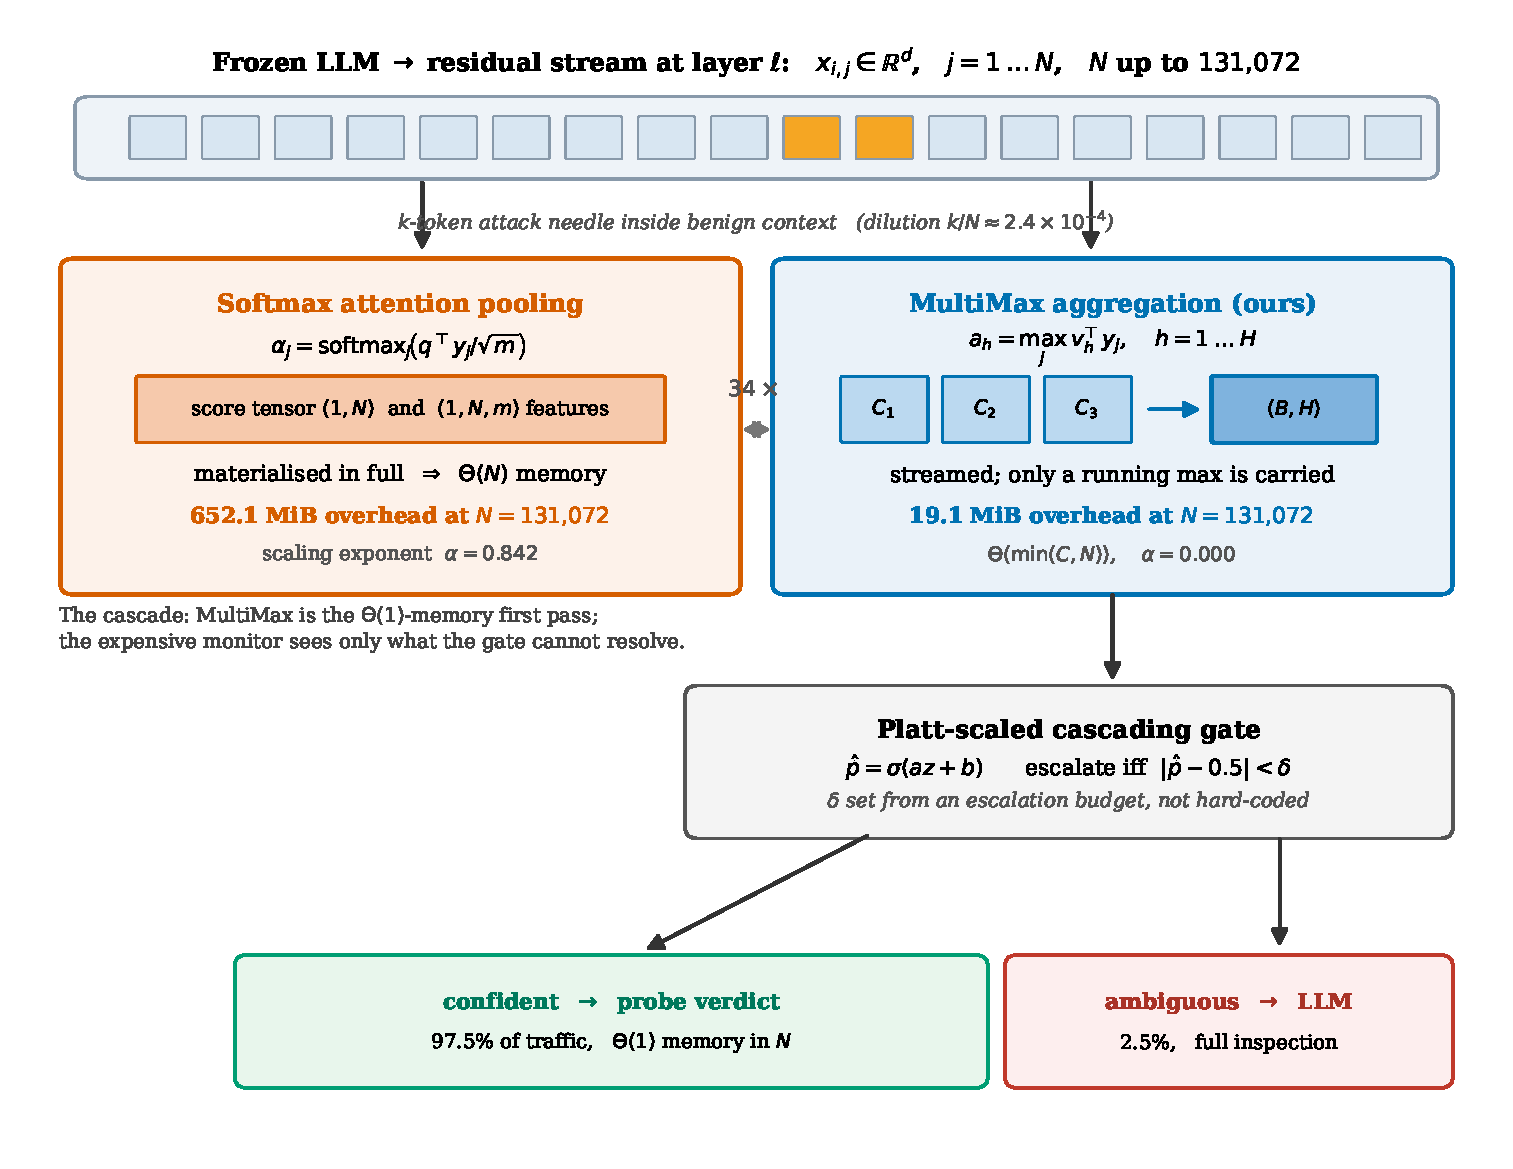
\includegraphics[width=\textwidth]{figures/fig1_architecture.pdf}
\caption{Aggregation as the independent variable, and the cascade it enables. Softmax
pooling materialises a score tensor over the sequence; MultiMax streams a per-head maximum
and carries only $(B,H)$ state. The Platt-scaled gate routes confident traffic to the
probe verdict and escalates only the ambiguous band.}
\label{fig:arch}
\end{figure}

\subsection{Benchmark A: systems scaling}
\label{sec:systems}
\begin{figure}[t]
\centering
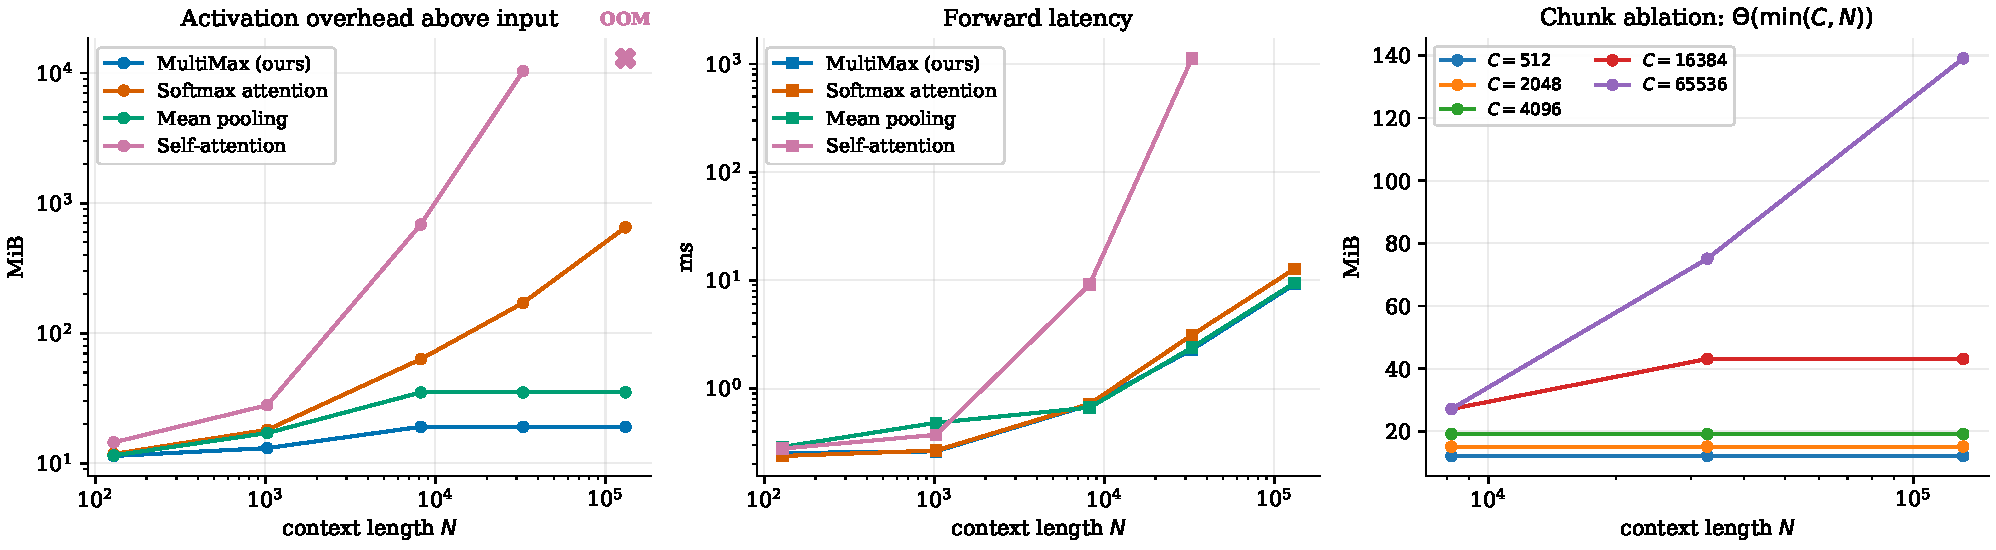
\includegraphics[width=\textwidth]{figures/fig2_memory_scaling.pdf}
\caption{Left, centre: activation overhead above the input tensor, and forward latency,
versus $N$. Right: the chunk ablation --- rows are flat in $N$ once chunking engages,
columns rise with $C$.}
\label{fig:memory}
\end{figure}

\begin{table}[t]
\centering\small
\begin{tabular}{lrrrrr}
\toprule
Probe & $N{=}8{,}192$ & $N{=}32{,}768$ & $N{=}131{,}072$ & overhead @131k & $\alpha$\\
\midrule
MultiMax (ours) & $0.707$\,ms & $2.293$ & $\mathbf{9.205}$ & $\mathbf{19.1}$\,MiB & $\mathbf{0.000}$\\
Mean pooling    & $0.667$ & $2.392$ & $9.438$ & $35.1$\,MiB & $0.000$\\
Softmax attention & $0.720$ & $3.125$ & $12.729$ & $652.1$\,MiB & $0.842$\\
Self-attention  & $9.182$ & $\mathbf{1128.474}$ & \textbf{OOM} & $10381.6$\,MiB & $1.960$\\
\bottomrule
\end{tabular}
\caption{Latency and activation overhead. $\alpha$ is the log--log exponent of overhead in
$N$, fitted on $N\ge8192$. Overhead excludes the input tensor, which is unavoidably
$\Theta(N)$ and would otherwise dominate.}
\label{tab:memory}
\end{table}

MultiMax overhead is flat at $19.1$\,MiB across a $16\times$ length increase
(Table~\ref{tab:memory}). Self-attention is $492\times$ slower than MultiMax at
$N{=}32{,}768$ and then exhausts memory. We note a correction to a common framing:
\emph{single-query} attention pooling is $\Theta(N)$, not $\Theta(N^2)$; its score tensor
is $(1,N)$. Only self-attention is quadratic.

\begin{remark}[Is $\mathcal{O}(1)$ real, or an artifact of chunking?]
\label{rem:complexity}
A reviewer should press on this, and the honest answer is that the suspicion is half
right. The flat footprint \emph{is} a consequence of streaming --- that is the mechanism,
not an artifact --- and it obeys a measurable law. Sweeping $C\times N$
(Fig.~\ref{fig:memory}, right) gives row spread exactly $0.0$\,MiB for every $C<N$
($\alpha=0.000$ at $C\in\{512,2048,4096\}$ across $N$ from $8{,}192$ to $131{,}072$),
while overhead rises with $C$ ($\beta=0.510$). For $C\ge N$ there is one chunk and the
chunk \emph{is} the sequence, so overhead tracks $N$ by construction. The law is
$\Theta(\min(C,N))$. The memory is not free; it is $\Theta(C)$ memory the operator
chooses, and $\Theta(1)$ in $N$, the one quantity the adversary controls.
\end{remark}

\subsection{Benchmark B: weak-signal detection}
\begin{figure}[t]
\centering
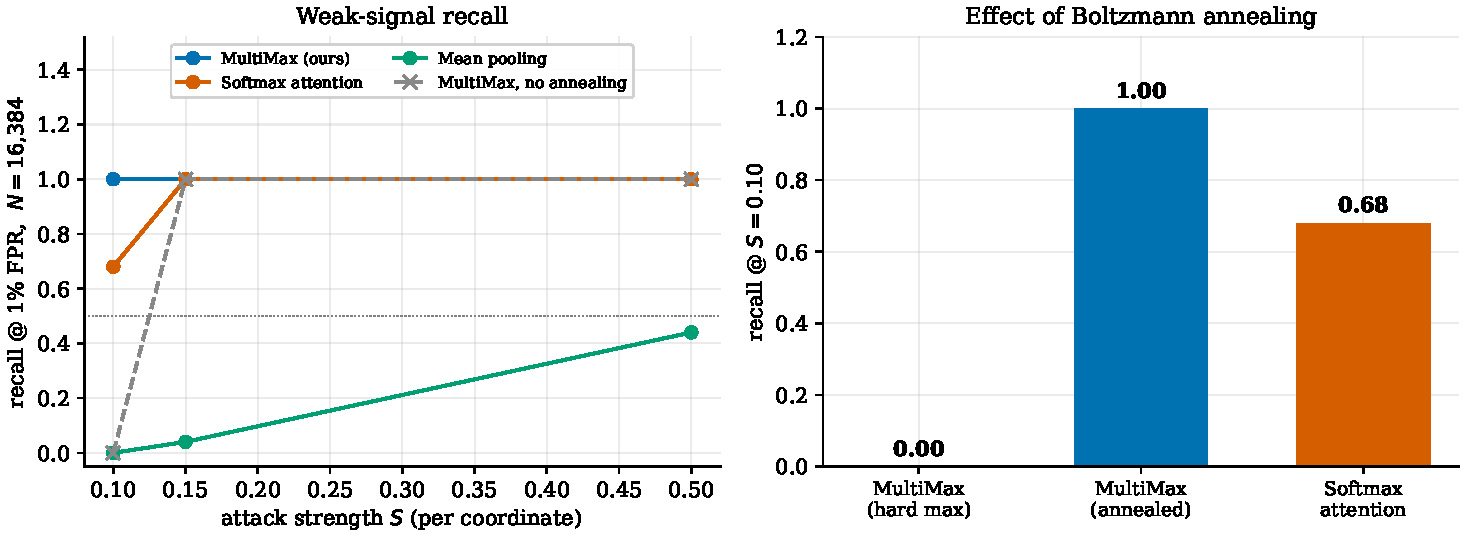
\includegraphics[width=0.92\textwidth]{figures/fig3_annealing_recall.pdf}
\caption{Recall at $1\%$ FPR, $N{=}16{,}384$, trained at $N{=}512$. Annealing converts a
total training failure at $S{=}0.10$ into full recall.}
\label{fig:anneal}
\end{figure}

\begin{table}[t]
\centering\small
\begin{tabular}{lccc}
\toprule
Strength $S$ & MultiMax (ours) & Softmax attention & Mean pooling\\
\midrule
$0.10$ & $\mathbf{1.00}\,/\,1.00$ & $0.68\,/\,1.00$ & $0.00\,/\,0.52$\\
$0.15$ & $1.00\,/\,1.00$ & $1.00\,/\,1.00$ & $0.04\,/\,0.94$\\
$0.50$ & $1.00\,/\,1.00$ & $1.00\,/\,1.00$ & $0.44\,/\,1.00$\\
\bottomrule
\end{tabular}
\caption{Recall@$16{,}384$ / recall@$512$. The second entry separates ``never learned the
concept'' from ``learned it, then diluted''. Dilution ratio $k/N=2.4\times10^{-4}$.}
\label{tab:recall}
\end{table}

With annealing, MultiMax attains full recall at every strength and leads softmax pooling
in the weak-signal regime ($1.00$ vs $0.68$ at $S{=}0.10$). Mean pooling never recovers,
as Prop.~\ref{prop:mean} requires. Without annealing the same architecture scores
$0.00/0.00$ at $S{=}0.10$: the gap between the two MultiMax rows in
Fig.~\ref{fig:anneal} is the entire contribution of \S\ref{sec:annealing}.

\subsection{Benchmark C: distributed attacks}
\label{sec:distributed}
\begin{figure}[t]
\centering
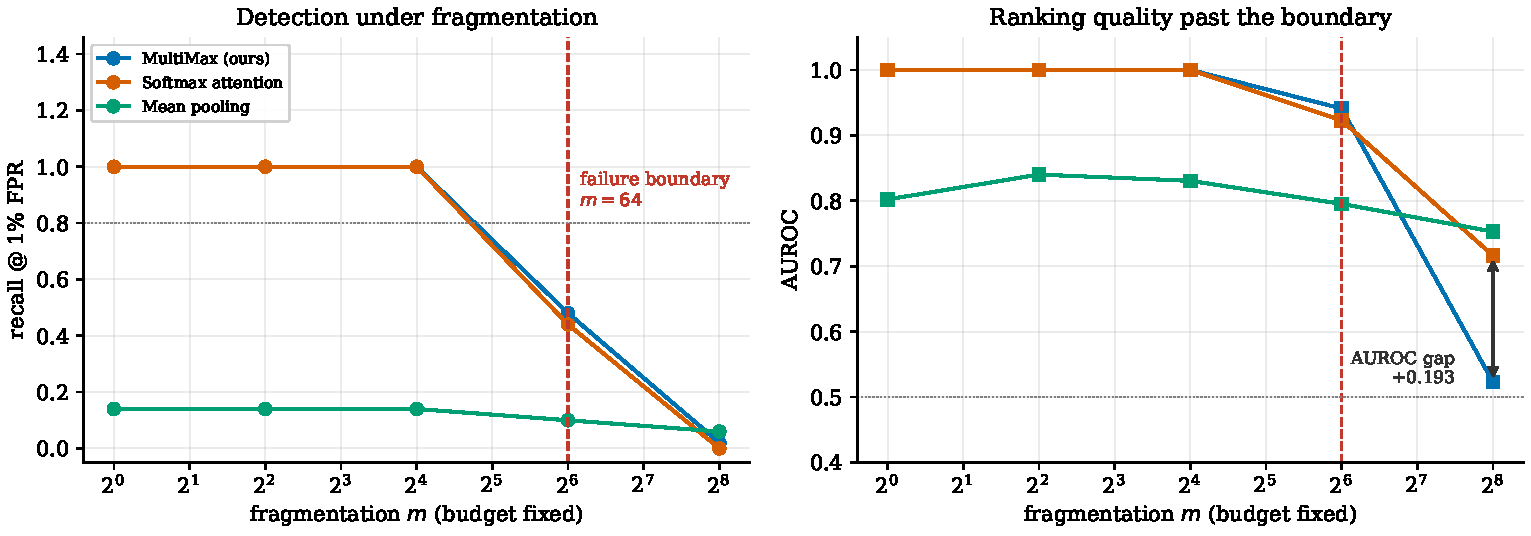
\includegraphics[width=0.95\textwidth]{figures/fig4_distributed_attack.pdf}
\caption{Fragmented attack: a fixed budget $S{=}2.0$ split across $m$ non-contiguous
tokens. Both pooled aggregators fail at $m{=}64$; past the boundary softmax retains
markedly better ranking.}
\label{fig:dist}
\end{figure}

An adversary who holds the total budget fixed but spreads it over $m$ non-contiguous
tokens presents per-token magnitude $S/m$, so
\begin{equation}
  \max_j v_h^\top y_j=\Theta(S/m),
  \qquad\text{while}\qquad
  \tfrac1N\textstyle\sum_j v_h^\top y_j=\Theta(S/N)\ \text{is unchanged in } m,
  \label{eq:distributed}
\end{equation}
the exact dual of Prop.~\ref{prop:mean}. This is the attack aimed at a maximum, and it is
the structural price of the hard reduction.

\begin{table}[t]
\centering\small
\begin{tabular}{rrccc}
\toprule
$m$ & per-token $S/m$ & MultiMax & Softmax attention & Mean pooling\\
\midrule
$1$   & $2.0000$ & $1.000$ & $1.000$ & $0.140$\\
$16$  & $0.1250$ & $1.000$ & $1.000$ & $0.140$\\
$64$  & $0.0312$ & $\mathbf{0.480}$ & $\mathbf{0.440}$ & $0.100$\\
$256$ & $0.0078$ & $0.020$ & $0.000$ & $0.060$\\
\bottomrule
\end{tabular}
\caption{Recall at $1\%$ FPR under fragmentation, $N{=}16{,}384$. Failure boundary
(recall $<0.80$): MultiMax $m{=}64$, softmax $m{=}64$, mean pooling $m{=}1$.}
\label{tab:distributed}
\end{table}

Two points, both against our own interest. First, the predicted MultiMax-specific
vulnerability \emph{did not isolate}: both pooled aggregators fail at the same $m$, so at
this budget the distributed attack degrades query-based pooling as much as the hard
reduction. Second, the recall boundary hides a real difference. At $m{=}256$ both sit at
recall $\approx0$ under a $1\%$ FPR threshold, but AUROC is $0.523$ for MultiMax against
$0.716$ for softmax: softmax keeps usable ordering after the thresholded detector has
failed, while the hard maximum loses its signal more completely.

% =====================================================================================
\section{Related Work}
% =====================================================================================
\paragraph{Probing and mechanistic interpretability.}
Linear probes on intermediate representations date to \citet{alain2016probes}. Recent
safety work trains them to detect deception \citep{goldowskydill2025deception} and
evaluates them at scale \citep{kretschmar2026liars,natarajan2026oneprobe}. A consistent
finding is that probes are strong in-distribution and brittle out of it
\citep{yoo2026subspace,boxo2025caught}. \citet{parrack2026blacktowhite} argue the right
metric is the \emph{black-to-white boost} over a black-box monitor, a standard we adopt.

\paragraph{Long-context guardrails.}
\citet{kramar2026gemini} deploy probes in a production assistant and report short-to-long
generalisation failure with architecture as a governing factor.
\citet{chen2026longguard} attribute the failure to attention dilution and logit-margin
compression. Our contribution is to isolate aggregation and give it a memory law.

\paragraph{Sparse dictionaries.}
Sparse autoencoders \citep{lieberum2024gemmascope} are an alternative route to
interpretable safety features, complicated by absorption \citep{chanin2024absorption} and
by the finding that they need not beat random baselines
\citep{korznikov2026sanity}. We deliberately avoid dictionary dependence.

\paragraph{Control and cascades.}
AI-control protocols pair trusted and untrusted monitors
\citep{greenblatt2023control,gardnerchallis2026untrusted}, and
\citet{koran2026ensemble} show diverse monitor ensembles outperform homogeneous ones at
equal compute. Our cascade is the low-latency first stage such protocols assume but rarely
characterise. Calibration follows \citet{platt1999probabilistic,guo2017calibration}; the
smooth-max operator is that of \citet{asadi2017boltzmann}; the straight-through estimator
is \citet{bengio2013estimating}.

% =====================================================================================
\section{Discussion, Rebuttal Analysis, and Limitations}
% =====================================================================================
\paragraph{What we do and do not claim.}
Combining Props.~\ref{prop:mean}--\ref{prop:softmax}, Rem.~\ref{rem:sparsity} and
\S\ref{sec:distributed}: against mean aggregation, MultiMax wins unconditionally on
concentrated attacks. Against single-query softmax pooling the advantage is conditional
and narrow --- $\gamma$ in Prop.~\ref{prop:softmax} is a \emph{trained} quantity, and a
salient needle drives $e^{\gamma}\!\sim\!N/k$, cancelling the dilution; post-annealing
MultiMax leads only in the weak-signal regime and ties elsewhere. Against a distributed
adversary the two fail together, with MultiMax degrading less gracefully. The
unconditional advantage is therefore the systems one, and the deployment recommendation
follows from it: use MultiMax as a $\Theta(1)$-memory first pass, not as a replacement for
inspection.

\paragraph{Rebuttal analysis.}
Two objections shaped this paper. (i) \emph{``Softmax outperforms MultiMax at $m{=}256$.''}
Correct on AUROC ($0.716$ vs $0.523$), and we report it in the abstract rather than the
appendix; it is why our claim is architectural rather than a detection claim.
(ii) \emph{``Is $19.1$\,MiB truly $\mathcal{O}(1)$?''} Half right, and it prompted the
chunk ablation of Rem.~\ref{rem:complexity}, which replaces an $\mathcal{O}(1)$ assertion
with the measured law $\Theta(\min(C,N))$.

\paragraph{Limitations.}
\emph{Synthetic activations.} Benchmarks run on Gaussian backgrounds with a single fixed
additive attack direction; real misuse features are neither isolated nor axis-aligned, and
the transfer of these results to real residual streams is untested.
\emph{Known-$m$ training.} Benchmark C trains on the same fragmentation it evaluates,
which is generous to the defender; an unknown-$m$ adversary is untested.
\emph{Threshold drift.} Rem.~\ref{rem:fpr} predicts $\sqrt{2\log N}$ growth in the benign
maximum; our protocol recalibrates per length by construction and does not characterise
the drift itself.
\emph{Simulated escalation.} The cascade's second stage is a deterministic stand-in
exercising routing and cost arithmetic; it is not evidence about a real monitor, and the
cost constants are illustrative.
\emph{Single scale.} One width, one head count, one GPU.

\paragraph{Reproducibility.}
Every number in this paper is read from a single JSON artifact produced by the benchmark
suite, and a checker verifies each quoted figure against it. This is not incidental: three
figures in an earlier draft had silently gone stale after a bug fix changed the underlying
model, and the checker exists because prose is not otherwise tested.

\bibliographystyle{plainnat}
\bibliography{references}

\end{document}
